% !TeX spellcheck = en_US 
\section{Method}\label{interlocking:sec:method}
This paper considers topologically interlocking structures satisfying extrusion continuity constraints,
which will be optimized for tensile strength;
the geometry of the designs are optimized to yield or break at the highest horizontally applied tensile stress.
The highest administrable force applied to a unit cell of any interlocking structure will be carried by both materials $a$ and $b$.
In the plane where tensile failure of material $a$ occurs the total force $F$ will be distributed over the cross-sectional area $A_a$;
likewise for material $b$.
The theoretically optimal interlocking microstructure would be such that the force $F$ will be homogeneously distributed over $A_a$ and $A_b$
in such manner that both materials will fail at the same ultimate force: $F = \sigmafail{a} A_a = \sigmafail{b} A_b$.
\revise{The structure will break where the force is distributed of the smallest area $A_a$ or $A_b$, so increasing their overall size would improve on the microstructure,
but}{The ultimate force before material $a$ breaks can be improved by increasing the area $A_a$, but this is at the cost of material $b$ (and vice versa), since} their combined area is limited to the total cross sectional area $A_\text{total}$ of the microstructure.
The ultimate strength of any multi-material microstructure is therefore limited to:

\begin{align}
	\sigma^* &= \frac{F}{A_\text{total}} 
	= \frac{F}{A_a + A_b}  \nonumber
	= \frac{\sigmafail{a} A_a}{A_a + A_b} \nonumber \\
	% = \frac{\sigmafail{b} A_b}{A_a + A_b} \nonumber \\
	%
	%\sigmafail{a} A_a &= \sigmafail{b} A_b \nonumber \\
	A_a &=  A_b \nicefrac{\sigmafail{b}}{\sigmafail{a} } \nonumber \\
\label{interlocking:eq:general_uper_bound}
	\sigma^*
	&= \frac{\sigmafail{a} A_b \nicefrac{\sigmafail{b}}{\sigmafail{a} } }{A_b \nicefrac{\sigmafail{b}}{\sigmafail{a} }  + A_b}
	%= \sigmafail{a} \frac{ \nicefrac{\sigmafail{b}}{\sigmafail{a} } }{ \nicefrac{\sigmafail{b}}{\sigmafail{a} }  + 1} \\
	%&= \frac{ \sigmafail{b} }{ \nicefrac{\sigmafail{b}}{\sigmafail{a} }  + 1} \\
	= \frac{ 1 }{ \nicefrac{1}{\sigmafail{a}} + \nicefrac{1}{\sigmafail{b}} } 
	%\approx \SI{8.6}{\mega\pascal} \text{ for PLA and PP}
\end{align}


This formula for the ultimate tensile strength of interlocking microstructures is a theoretical upper bound.
In practice the worst cross-sectional area $A_a$ is in a different plane than the worst cross-sectional area $A_b$, so they do not add up to $A_\text{total}$.
For example, in the dovetail geometry (\cref{interlocking:fig:basic_2d_interlock}) the highest stress of a dovetail of material $a$ is at its base, while the highest stress in $b$ will be at the end of the dovetail of material $a$.
The geometry by which the interlock is secured reduces the strength compared to the theoretical upper bound of the ultimate tensile strength.
The upper bound can therefore never be reached.
% Moreover, the stress distribution will be heterogeneous when subjecting a complex geometry to tension.







\begin{figure*}
	\centering
	\begin{subfigure}[B]{.32\textwidth}
		\centering
		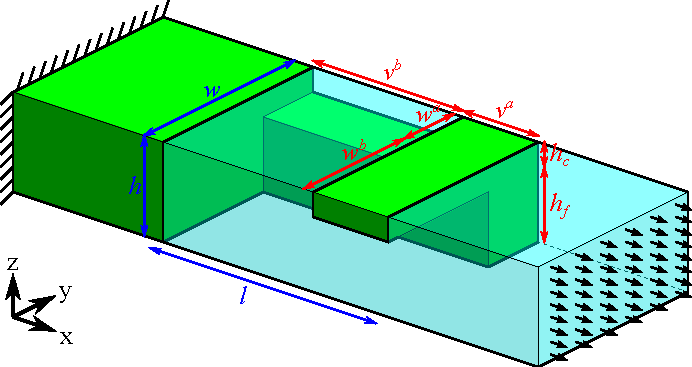
\includegraphics{sources-method-straight_model_v5_no_failures.pdf}
		\caption{Design variables (in red)}
		\label{interlocking:fig:straight_model}
	\end{subfigure}
	\begin{subfigure}[B]{.32\textwidth}
		\centering
		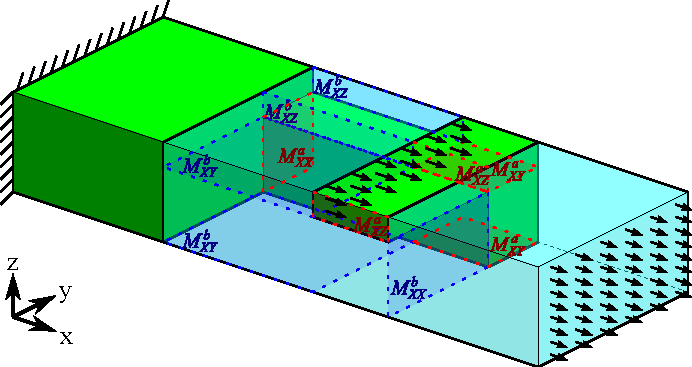
\includegraphics{sources-method-straight_model_v5_failures.pdf}
		\caption{Failures modes for material $a$ (in red) and for $b$ (in blue)}
		\label{interlocking:fig:straight_model_failure_modes}
	\end{subfigure}
	\begin{subfigure}[B]{.32\textwidth}
		\centering
		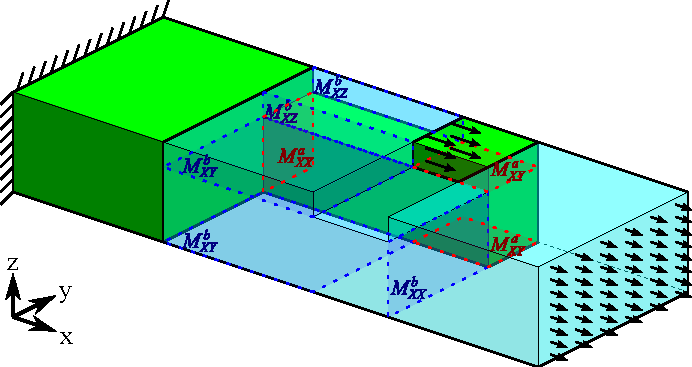
\includegraphics{sources-method-straight_model_v5_broken.pdf}
		\caption{Partly broken, partly interlocking cell}
		\label{interlocking:fig:straight_model_broken}
	\end{subfigure}
	\caption{Unit cell of the straight ITIM variant. Force is transferred from material $a$ (green) to material $b$ (transparent cyan) through the contact area on the cross beams. In the partly broken situation there is still interlocking, but the total force is transferred through a narrower area.}
\end{figure*}

\begin{figure*}
	\centering
	\begin{subfigure}[B]{.25\textwidth}
		\centering
		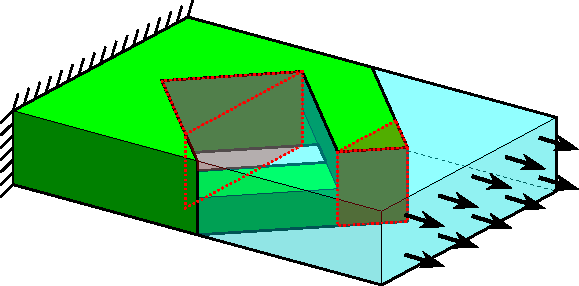
\includegraphics{sources-method-diagonal_model_simple_v5.pdf}
		\caption{Simple cell}
		\label{interlocking:fig:diagonal_model_simple}
	\end{subfigure}
	\begin{subfigure}[B]{.33\textwidth}
		\centering
		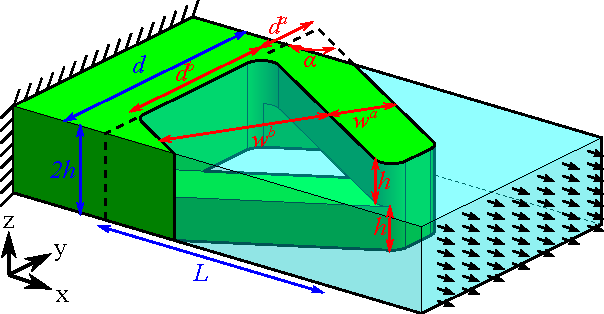
\includegraphics{sources-method-diagonal_model_v5_no_failures.pdf}
		\caption{Rounded and aligned design}
		\label{interlocking:fig:diagonal_model}
	\end{subfigure}
	\begin{subfigure}[B]{.33\textwidth}
		\centering
		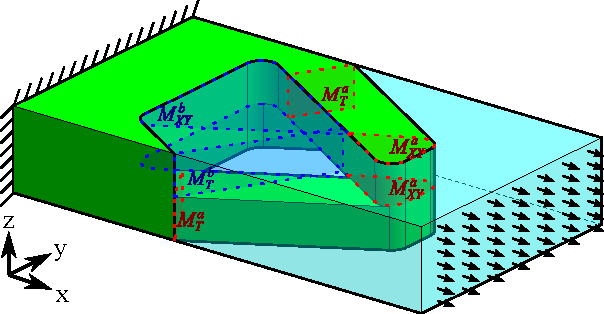
\includegraphics{sources-method-diagonal_model_v5_failures.pdf}
		\caption{Failure modes}
		\label{interlocking:fig:diagonal_model_failures}
	\end{subfigure}
	\caption{Unit cell of the diagonal ITIM variant. The $\mt{m}$ failure modes are orthogonal to the beams and influenced by both tensile and shear components of the total force.}
\end{figure*}




\subsection{Interlaced Topologically Interlocking Microstructure}\label{interlocking:sec:itim}
The topologically interlocking structure we propose consists of horizontal beams alternating in material.
On top of that we print another set of beams rotated about Z and on top beams of the first rotation again, etc.
Long horizontal beams assure continuous extrusion, while the alternating direction of the beams assures the interlock.
See \cref{interlocking:fig:basic_structure_single_mat}.


When joining bodies of different materials, some region around the interface between the two bodies should be replaced by a number of unit cells from such a lattice structure.
The length of the transition region $L$ is limited by the design of the product within which the lattice is to be employed.
We consider a design constraint of $\lmax = 12 \wmin{m} = \SI{3.6}{\milli\meter}$;
this is enough to have some design freedom for the microstructure, while limiting the impact on the rest of the product.

With a relatively small length $\lmax$ it stands to reason to fill that space using a single unit cell in the length direction only.
If the same region were to be filled with 2 versions of the same cell but scaled to half lengthwise, then the total area of shear remains the same,
but the shear areas of the two cells would not bear the same load, so the stresses in one of the cells would only increase by using two cells instead of one.
One might consider using a different geometry for the two cells to counteract that fact,
but we do not expect such a multi-layered interlocking design to outperform a single layered interlocking lattice when $\lmax$ is relatively low. 

\revise{Given that we will fill the space around the interface with a single layer of cells, the orientation of those cells w.r.t. the interface is relevant.}{According to the reasoning above we should fill the interface with a single layer of cells, but how should those cells be oriented w.r.t. the interface?}
While rotating the lattice about X or Y is impossible due to the continuous extrusion constraint, we are free to rotate about Z.
However, given that the tensile stress is applied in a single direction it only makes sense to consider two orientations: straight and diagonal.


For the materials chosen by this study, Ultimaker Tough \revise{PLA}{Polylactic Acid} (\revise{T}{}PLA) and Ultimaker PolyPropylene (PP), the theoretical upper bound comes out to be \SI{8.6}{\mega\pascal}.
The structure may not only be subject to tensile failure, but also to shear failure modes.
Because of the layer-wise build-up employed by \revise{FDM}{MEX}, the tensile properties in the Z direction are different from those in the horizontal plane.
See \cref{interlocking:tab:mat_props_manufacturing_constraints}.
The structure is furthermore subject to manufacturing constraints determined by the nozzle sizes and the layer thickness.
The standard layer thickness $\hmin$ is \SI{0.1}{\milli\meter} and the minimal line width $\wmin{}$ for a \SI{0.4}{\milli\meter} nozzle is \SI{0.3}{\milli\meter}.


\begin{table}
	\caption{Yield properties of single material \revise{FDM}{MEX} printed samples.}
	\label{interlocking:tab:mat_props_manufacturing_constraints}
	\centering
	\begin{tabular}{l|rrrrrr}
		material & $\sigmafail{}$ & $\sigmafailz{}$ & $\epsilon_\text{y}$ & $\epsilon_\text{yZ}$ \\
		\hline
		\revise{T}{}PLA & \SI{47}{\mega\pascal} & \SI{33}{\mega\pascal} & \SI{3.5}{\percent} & \SI{2.6}{\percent}\\
		PP & \SI{10.5}{\mega\pascal} & \SI{10.6}{\mega\pascal} & \SI{29}{\percent} & \SI{22}{\percent}
	\end{tabular}
\end{table}


If all dimensions of the beams are set to minimal and the angle between the beams is set to \SI{90}{\degree},
%tensile tests show that the straight ITIM variant reaches \SI{3.3}{\mega\pascal} and the diagonal variant reaches \SI{4.9}{\mega\pascal}.
the finger of the straight ITIM variant takes up a quarter of the area at the base of the cell, so we can expect the strength to be close to $\nicefrac14 \sigmafail{b} \approx \SI{2.6}{\mega\pascal}$.
For the diagonal ITIM variant the beams take up half of the area at the base of the cell, which would be close to $\nicefrac12 \sigmafail{b} \approx \SI{5.3}{\mega\pascal}$.
However, these ultimate strengths can be improved upon considerably by optimizing the geometry.
This section considers these two ITIM variants and analytical models to optimize them.




\subsection{Straight ITIM variant}
A unit cell of the straight ITIM variant is visualized in \cref{interlocking:fig:straight_model}.
A cell consists of a single \emph{finger} of height $\hf$ protruding from the body of material $a$ outward and part of a \emph{cross beam} of height $\hc$ angled at \SI{90}{\degree}.
In order to print the relatively short fingers using continuous extrusion, we employ the constraints that $\wm \ge 2\wmin{m}$ (where $m$ is either material $a$ or $b$),
so that the toolpaths for the outline of each layer can go back and forth along the finger without interruption.
The cross beams are long and continuous enough, so they could be printed using a single extrusion path: $\vm \ge \wmin{m}$.
We set the minimum height of the beams to twice the layer height, so as to be able to recover from manufacturing inaccuracies\footnote{If the structure would consist of alternating geometry each layer, then the inaccuracy of the one layer can cause over-extrusion in the next layer,
	which snowballs the problem upward during printing.}: $\hf \ge 2\hmin$ and $\hc \ge 2\hmin$.


%\subsubsection{Straight ITIM variant (whole)}
In order to optimize the straight ITIM variant for a maximal tensile strength we consider three types of stress, related to three types of failure mode for either material $m$:
tensile stress $\stresstensile{m}$ for $\myz{m}$, cross beam shear stress $\stresscrossshear{m}$ for $\mxz{m}$ and Z shear stress $\stresszshear{m}$ for $\mxy{m}$.
See \cref{interlocking:fig:straight_model_failure_modes}.
These three types of failure mode for either material are modelled using classical beam theory as having a homogenous stress distribution.
Because the total force $F$ is modelled as being homogeneously distributed over the whole cross beam,
the two shear stresses obtain only a portion of the total force.
Furthermore, they are divided by two because the beams and pillars are fixed on both sides:
%The Z shear stress $\stresszshear{m}$ is multiplied with the ratio between the vertical and horizontal strength, so that all stresses can be compared to $\sigmafail{m}$ fairly.

\begin{align}
	\stresstensile{m} &= \frac{ F }{ \wm \hf } \label{interlocking:eq:tensile} \\
	\stresscrossshear{m} &= \frac{\w{\neg m}}{w} \frac{ F}{2 \vm \hc} \label{interlocking:eq:cross_shear} \\
	%	\stresszshear{m} &= \frac{\sigmafail{m}}{\sigmafailz{m}} \frac{\w{m}}{w}  \frac{ F }{ 2 \vm \wm} \label{interlocking:eq:z_shear} \\
	\stresszshear{m} &= \frac{\w{m}}{w}  \frac{ F }{ 2 \vm \wm} \label{interlocking:eq:z_shear} \\
	\text{where } & m \in \left\{ a, b \right\} \text{ and } \neg a = b \text{ and } \neg b = a  \nonumber
\end{align}



\begin{figure}
	\begin{tcolorbox}[colback=white,title=Model of the straight ITIM variant]
		\begin{align}
			f: & \max{ \frac{F}{\left( \wa + \wb \right) \left( \hf + \hc \right) } }  \label{interlocking:eq:objective} \\
			\omit\rlap{subject to} \nonumber \\
			\gwb: & \wb \ge 2 \wmin{b} 		&&	\label{interlocking:eq:gwb}\\
			\gva: & \va \ge \wmin{a} 		&&	\label{interlocking:eq:gva}\\
			\gvb: & \vb \ge \wmin{b} 		&&	 \label{interlocking:eq:gvb}\\
			\ghf: & \hf \ge \hmin 		&&	 \label{interlocking:eq:ghf}\\
			\gtm: & \frac{ F }{ \wm \hf } \le \sigmafail{m} &&	\myz{m}  \label{interlocking:eq:g_tensile_a} \\
			%\gtb: & \frac{ F }{ \wb \hf  } \le \sigmafail{b} &&	\myz{b}  \label{interlocking:eq:g_tensile_b} \\
			\gca: & \frac{\wb}{w} \frac{ F }{ 2 \va \hc  } \le  \frac{1}{\sqrt{3}} \sigmafail{a} &&	 \mxz{a}  \label{interlocking:eq:g_shear_a} \\
			%\gza: & \frac{\wa}{w} \frac{ F }{ 2 \va \wa  } \le  \frac{1}{\sqrt{3}} \sigmafailz{a} 	&&	 \mxy{a} \label{interlocking:eq:g_z_shear_a} \\
			\gzm: & \frac{\wm}{w} \frac{ F }{ 2 \vb \wb  } \le  \frac{1}{\sqrt{3}} \sigmafailz{m} 	&&	\mxy{b} \label{interlocking:eq:g_z_shear_b} \\
			\omit\rlap{where \cref{interlocking:eq:g_tensile_a,interlocking:eq:g_z_shear_b} are duplicated  } \nonumber \\ 
			\omit\rlap{for both materials $ m \in \left\{a, b\right\} $ } \nonumber
		\end{align}
	\end{tcolorbox}
\end{figure}


The tensile stress of the whole cell is given by $\nicefrac{F}{(\wa +\wb)(\hf + \hc)}$.
Combining the above we obtain the constrained optimization problem given by \crefrange{interlocking:eq:objective}{interlocking:eq:g_z_shear_b}.
The $\sqrt{3}$ in \cref{interlocking:eq:g_shear_a,interlocking:eq:g_z_shear_b} comes from the von Mises yield criterion.
Although one might consider combining the stresses together using the same criterion, this does not increase the accuracy of the model,
because the failure mode planes do not overlap.

Because the objective and all stresses are invariant under various scaling operations,
we can choose the value of a subset of the design variables.
Because of invariance to uniform scaling we employ the design constraint;
scaling up the width and force only increases the cross beam shear values $\stresscrossshear{m}$, so we employ the minimum width constraint;
scaling up the height and force only increases the Z shear values $\stresszshear{m}$, so we employ the minimum height constraint.
This way we limit the design space from six to three dimensions, i.e. $\wb, \hf, \va$:
\begin{align}
	\wa &= 2 \wmin{a}   & %\label{interlocking:eq:wa} \\
	\hc &= 2\hmin  & %\label{interlocking:eq:hc}\\
	\vb &= \lmax - \va \label{interlocking:eq:va}
\end{align}




Using the formulae of the constrained optimization problem one can find the maximum force and thus the maximum stress of any design;
we can rewrite each of the mechanical constraints \crefrange{interlocking:eq:g_tensile_a}{interlocking:eq:g_z_shear_b} to give a formula for $F$
and the lowest value of those formulae will give the active failure mode for a given design.
The resulting response surfaces are shown in \cref{interlocking:fig:analytic_response_whole}.
The optimum is at the intersection of four constraint surfaces, which is remarkable for a 3D space.


\begin{figure}
	\centering
	\begin{subfigure}[B]{\columnwidth}
		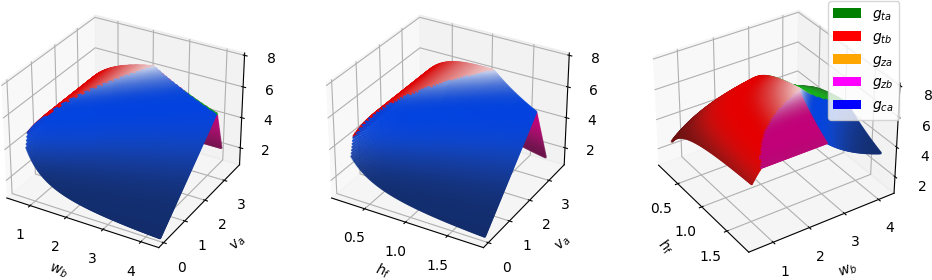
\includegraphics{sources-method-analytic_response_whole_bigger_fonts.png}
		\caption{Straight ITIM model response. At $\hf = 1.29$, $\wb=2.64$ and $\va=2.70$ respectively.}
		\label{interlocking:fig:analytic_response_whole}
	\end{subfigure}
	\begin{subfigure}[B]{\columnwidth}
		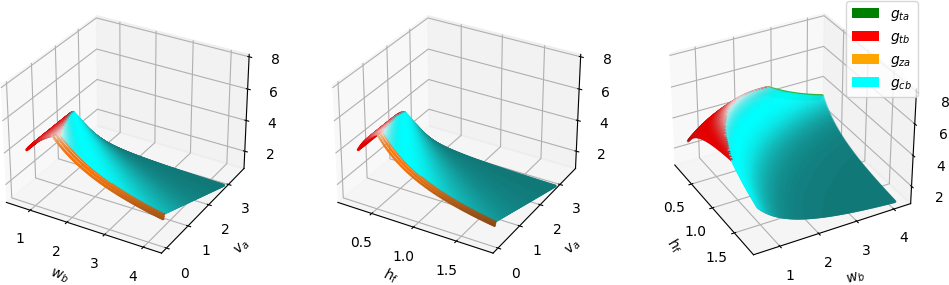
\includegraphics{sources-method-analytic_response_broken_bigger_fonts.png}
		\caption{Straight ITIM model response (broken). At $\hf = 0.50$, $\wb=1.50$ and $\va=0.36$ resp.}
		\label{interlocking:fig:analytic_response_broken}
	\end{subfigure}
	\caption{Maximum strength according to analytical models for the straight ITIM variant along three 2D slices of the 3D design space.
		Four constraint surfaces meet at the optimum.
		By taking the maximum values of these two models the maximum stress before separation can be calculated.
	}
	\label{interlocking:fig:analytic_response}
\end{figure}













\subsubsection{Broken cross beams model}
A careful analysis of the geometry will show that if shear failure $\mxz{a}$ has occurred, 
there is still interlocking between the two materials. 
If a part of the cross beams of $a$ has sheared off, still the pillar of material $a$ remains, which is surrounded by material $b$.
See \cref{interlocking:fig:straight_model_broken}.
Once failure mode $\mxz{a}$ has occurred, still any other failure mode has to occur for the interlock to fail completely.
Since the failure mode can only happen by part of the PP cross beam pushing against the part of the \revise{T}{}PLA cross beam which is being sheared off,
both cross beams shear together.
Because \revise{T}{}PLA breaks at a lower strain than PP (see \cref{interlocking:tab:mat_props_manufacturing_constraints}), we know that for these materials $\mxz{b}$ never occurs unless $\mxz{a}$ has occurred.
We will construct a separate model for analysing the case where the \revise{T}{}PLA cross beam is broken into segments.


Because part of the cross beam is missing the stress on the remaining part increases.
Moreover, the cross beam shear constraint for PP ($\gcbbroken$) comes into play and the Z shear constraint $\gzb$ and the cross beam shear constraint $\gca$ are dropped because of the change in the cross beam of $a$.
The shear constraints \crefrange{interlocking:eq:g_shear_a}{interlocking:eq:g_z_shear_b} are replaced by \cref{interlocking:eq:g_shear_b_broken,interlocking:eq:g_z_shear_a_broken}.

\begin{figure}
\begin{tcolorbox}[colback=white,title=Straight ITIM variant - shear constraints for broken case]
	\begin{align}
		\gcbbroken: & \frac{ F }{ 2 \left( \lmax - \va \right) 2 \hmin } \le  \frac{1}{\sqrt{3}} \sigmafail{b} &&	 \mxz{b}  \label{interlocking:eq:g_shear_b_broken} \\
		\gzabroken: & \frac{ F }{ 2 \va \wa } \le \frac{1}{\sqrt{3}} \sigmafailz{a}  	&&	 \mxy{a} \label{interlocking:eq:g_z_shear_a_broken}
	\end{align}
\end{tcolorbox}
\end{figure}
The response surface of this model is shown in \cref{interlocking:fig:analytic_response_broken}.
In order to estimate the ultimate force of a given design one must consider both of these models: the one for the whole and the one for the broken situation.
When considering designs where the cross beam constraint $\gca$ is active in the whole model, the maximal force applicable is the highest of the two maximal forces according to the two models.















\subsection{Diagonal ITIM variant}
Besides the straight variant of the ITIM lattice, we also consider the variant where the beams are oriented diagonally to the interface surface.
\Cref{interlocking:fig:diagonal_model_simple} shows a simple cell of the ITIM lattice in the diagonal orientation.
Because the stress applied is homogeneous and precisely normal to the interface the optimal structure should be symmetric.
Due to symmetry there is no distinction between fingers and cross beams to be made in this model.
Both beams should have the same height $2\hmin$ and the angle $\alpha$ between the beams and the interface of both beams is the same.
The remaining design variables are: $\wa$, $\wb$ and $L$.

The simple cell consists of protruding fingers and triangular dents (see red triangles in \cref{interlocking:fig:diagonal_model_simple});
however, the advantage these dents give to the strength of the pattern is vastly outweighed by their effect on the total length $L$.
We therefore trim the triangular ends on the pattern to arrive at the model shown in \cref{interlocking:fig:diagonal_model}.
However, doing this introduces some sharp edges, with a diameter below the minimum feature size $\wmin{}$.
We therefore round the vertical edges using a radius $r=\SI{0.15}{\milli\meter}$
and define the dimensions of the model such that the rounded edges at the ends of both fingers are aligned.
See \cref{interlocking:fig:analytical_math_diagonal}.


Because of the diagonal geometry we expect that the stress distribution throughout the structure will be quite complex,
and the failure will depend on the deformation of both materials during stretching.
Nevertheless, we provide a simplified analytical model assuming the stress is homogeneously distributed and disregarding the influence of deformation on stress distribution.
We decompose the force $F$ into one component parallel and another orthogonal to the direction of the beams.
We then use the parallel component to determine the tensile stress and the orthogonal component to determine the shear stress in the beam,
which combine into a single constraint using the von Mises yield criterion in \cref{interlocking:eq:g_tensile_m_diag}.
The diagonal ITIM model is then defined by the constrained optimization problem given by \crefrange{interlocking:eq:objective_diagonal}{interlocking:eq:g_z_shear_m_diag}.



\begin{figure}
	\begin{tcolorbox}[colback=white,title=Model for the diagonal ITIM variant]
	\begin{align}
		f: & \max{ \frac{F}{ 2h d } }  \label{interlocking:eq:objective_diagonal} \\
		\omit\rlap{subject to} \nonumber \\
		\gwa: & \wa \ge 2\wmin{a}		&&	\label{interlocking:eq:gwa_diag}\\
		\gwb: & \wb \ge 2\wmin{b}		&&	\label{interlocking:eq:gwb_diag}\\
		\gd:  & L \le \lmax && \label{interlocking:eq:gd_diag}\\
		\gtm: & \frac{ F }{ 2 \wm h } \sqrt{ \left( \frac{w}{d} \right)^2  + 3 \left( \frac{w}{2M} \right)^2 } \le \sigmafail{m} &&	\mt{m}  \label{interlocking:eq:g_tensile_m_diag} \\
		%\gtb: & \frac{ F }{ 2 \wb h } \sqrt{ \left( \left( \frac{w}{d} \right)^2  + 3 \left( \frac{d}{2M} \right)^2 \right) } \le \sigmafail{b} &&	\mt{b}  \label{interlocking:eq:g_tensile_b_diag} \\
		%\gtb: & \frac{ F }{ 2 \wb h } \sqrt{ \left( \left( \frac{w}{d} \right)^2  + 3 \left( \frac{d}{2M} \right)^2 \right) } \le \sigmafail{b} &&	\mt{b}  \label{interlocking:eq:g_tensile_b_diag} \\
		\gzm: & \frac{F}{2 A_{\text{z},m}} \le  \frac{1}{\sqrt{3}} \sigmafailz{m} 	&&	 \mxy{m} \label{interlocking:eq:g_z_shear_m_diag} \\
		%\gza: & \frac{F}{2 A_{\text{z},a}} \le \sigmafailz{a} 	&&	 \mxy{a} \label{interlocking:eq:g_z_shear_a_diag} \\
		%\gzb: & \frac{F}{2 A_{\text{z},b}} \le \sigmafailz{b} 	&&	 \mxy{b} \label{interlocking:eq:g_z_shear_b_diag} \\
		\omit\rlap{where} \nonumber \\
		d &= 2Mw / \sqrt{4M^2-w^2} \nonumber \\
		M &= L - 2r \nonumber \\
		w &= \wa + \wb \nonumber \\
		A_{\text{z},m} &= 	\rlap{$\frac12 \pi r^2 + r (\wm-2r) \frac{d}{w} + d M \left(\frac{\wm}{w}\right)^2$} \nonumber \\
		\omit\rlap{where \cref{interlocking:eq:g_z_shear_m_diag,interlocking:eq:g_tensile_m_diag} are duplicated  } \nonumber \\ 
		\omit\rlap{for both materials $ m \in \left\{a, b\right\} $ } \nonumber
	\end{align}
\end{tcolorbox}
\end{figure}




\iffalse
area of \revise{T}{}PLA under shear and tension: $\wa h$.
von Mises criterion:
\begin{align*}
	\left( \frac{ \nicefrac12 \nicefrac{w}{d} F }{ \wa h } \right)^2 + 3 \left( \frac{ \nicefrac12 \nicefrac{d}{2M} F }{ \wa h } \right)^2 &\le \sigmafail{a}^2 \\
	\left( \frac{ F }{ 2 \wa h } \right)^2 \left( \left( \frac{w}{d} \right)^2  + 3 \left( \frac{d}{2M} \right)^2 \right) &\le \sigmafail{a}^2 \\
	\frac{ F }{ 2 \wa h } \sqrt{ \left( \left( \frac{w}{d} \right)^2  + 3 \left( \frac{d}{2M} \right)^2 \right) } &\le \sigmafail{a} \\
	F \sqrt{ \left( \left( \frac{w}{d} \right)^2  + 3 \left( \frac{d}{2M} \right)^2 \right) } &\le 2 \sigmafail{a} \wa h \\
	F &\le \frac{ 2 \sigmafail{a} \wa h }{  \sqrt{ \left( \frac{w}{d} \right)^2  + 3 \left( \frac{d}{2M} \right)^2 } }  \\
\end{align*}


% NAIVE pp stress: area of PP under tension alone $\mt{b}$: $ 2h \frac{\wb}{w} d$. PP tensile stress: $\frac{\nicefrac12 F w}{\wb d 2 h} = \frac{F w}{4 \wb d h} \le \sigmafail{b}$
\fi


Again the stresses are all scale-invariant, so we set $\wa = 2 \wmin{a}$.
However, because changes in $\wb$ given the same $L$ will change the angle $\alpha$ of the beams, we cannot assume the design constraint $\gd$ is active.

The resulting response surface can be viewed in \cref{interlocking:fig:analytic_response_diagonal}.
Because the height of the fingers is minimal the Z shear constraints are both dominated.


\begin{figure}
	\centering
	\begin{subfigure}[B]{.4\columnwidth}
		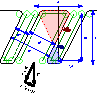
\includegraphics{sources-method-diagonal_math.pdf}
		\caption{Geometric relations.}
		\label{interlocking:fig:analytical_math_diagonal}
	\end{subfigure}
	\begin{subfigure}[B]{.59\columnwidth}
		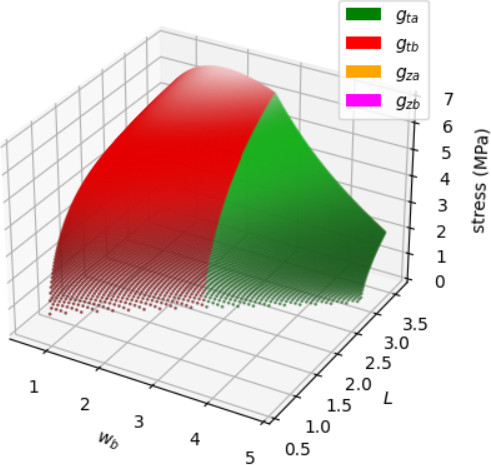
\includegraphics{sources-method-analytic_response_diagonal.jpg}
		\caption{Response surface coloured to failure mode.}
		\label{interlocking:fig:analytic_response_diagonal}
	\end{subfigure}
	\caption{Analytical model for the diagonal ITIM cell. The Z shear constraints are redundant because of the small height of the unit cell. The optimum is determined only by the tensile constraint of PP: $\gtb$.}
	%	\label{interlocking:fig:analytic_response}
\end{figure}


